\chapter{ETAT DE L'ART}
\begin{spacing}{1.2}
\minitoc
\thispagestyle{MyStyle}
\end{spacing}
\newpage

%----------------------------------------------------------------------------------------
%Notion de caméras	
%----------------------------------------------------------------------------------------
\section{INTRODUCTION}


Dans le cadre de l'étude de notre thème, il est essentiel de bien comprendre les concepts fondamentaux et les termes techniques qui sous-tendent ce domaine. Ce chapitre se propose de définir et d'expliquer les principaux mots-clés de notre thème, à savoir le calibrage, la caméra et la mesure de distance à l'aide d'une caméra. En démystifiant ces notions, nous établirons une base solide pour explorer les méthodes et les applications spécifiques de ces technologies dans le contexte de l'analyse des performances athlétiques.

Le calibrage, souvent utilisé de manière interchangeable avec l'étalonnage, fait référence à l'ensemble des processus et des techniques utilisés pour déterminer les paramètres intrinsèques et extrinsèques d'une caméra. Ces paramètres sont cruciaux pour corriger les distorsions optiques et pour transformer les coordonnées d'image en coordonnées réelles, assurant ainsi une mesure précise des distances et des angles.

Les caméras, quant à elles, sont des dispositifs optiques permettant de capturer des images ou des vidéos. Elles jouent un rôle central dans notre étude, car la qualité et la précision des données qu'elles fournissent dépendent en grande partie de leur bon calibrage.  

Enfin, la mesure de distance à l'aide d'une caméra est une application pratique du calibrage. Elle permet de convertir les informations bidimensionnelles capturées par la caméra en données tridimensionnelles, indispensables pour évaluer les performances des athlètes lors des sauts en longueur.  

En clarifiant ces concepts, nous poserons les bases nécessaires pour comprendre comment le calibrage ou l'étalonnage des caméras peuvent être appliqués efficacement à l'analyse des performances athlétiques, et en particulier à l'estimation des distances de saut en longueur.



 \newpage
 
 %----------------------------------------------------------------------------------------
 %Notion de caméras	
 %----------------------------------------------------------------------------------------
 
 \section{Notion de caméras}
 
 Une caméra est un dispositif qui capture la lumière et la transforme en image. Elle le fait à travers une lentille, qui concentre la lumière sur une surface sensible à celle-çi, où une image se forme \cite{noauthor_quest-ce_nodate}. Elle possède un micrologiciel ou "firmware" en anglais qui représente un type de logiciel programmer dans son matériel. Ce programme contrôle toutes les fonctions de la caméra, de la mise au point automatique et des paramètres d’exposition jusqu'au traitement et au stockage des images.
 
 Une caméra comprend les parties essentielles suivant: 
 \begin{itemize}
 	\item \textbf{Le corps :} qui tient l'ensemble de toutes les composantes . 
 	
 	\item \textbf{La lentille :} qui met la lumière au centre du capteur d’image. 
 	
 	\item \textbf{L’obturateur :} qui contrôle la quantité de lumière qui atteint le capteur.
 	
 	\item \textbf{L’ouverture :} qui contrôle la quantité de lumière que l’objectif laisse entrer.
 	
 	\item \textbf{Le capteur d'image:} qui convertit le rayonnement électromagnétique en un signal électrique analogique. Celui-çi est ensuite amplifié, puis numérisé par un convertisseur analogique-numérique et enfin traité pour obtenir une image numérique.  
 \end{itemize}
 
 Grâce à l'évolution continuelle de la technologie pour s'adapter aux demandes croissantes des consommateurs pour des images de haute qualité et des fonctionnalités innovantes, nous pouvons classer les caméras par catégories et par types.
 
 Il existe trois catégories de caméras qui sont entre autre \cite{noauthor_camera_2024}:
 \begin{itemize}
 	\item \textbf{Les caméras numériques}: qui capturent des images par voie électronique à l’aide d’un capteur.
 	
 	\item \textbf{Les caméra analogique}: qui enregistre ou transmet un signal électronique analogique. 
 	Ce signal est la partie de l'électronique qui exploite des signaux pouvant fonctionner ou être mesurés par des valeurs continues. 
 	
 	\item\textbf{caméra argentique}: qui utilise une bande de pellicule (Figure \ref{fig:Pellicule})enduit de produits chimiques photosensibles pour la réalisation de film cinématographique.
 	La pellicule est un support souple recouvert d'une émulsion contenant des composés sensibles à la lumière, généralement à base d'halogénures d'argent.
 	
 \end{itemize}
 
 \begin{figure}[H]%
 	\center%
 	\setlength{\fboxsep}{5pt}%
 	\setlength{\fboxrule}{0.5pt}%
 	\fbox{
 		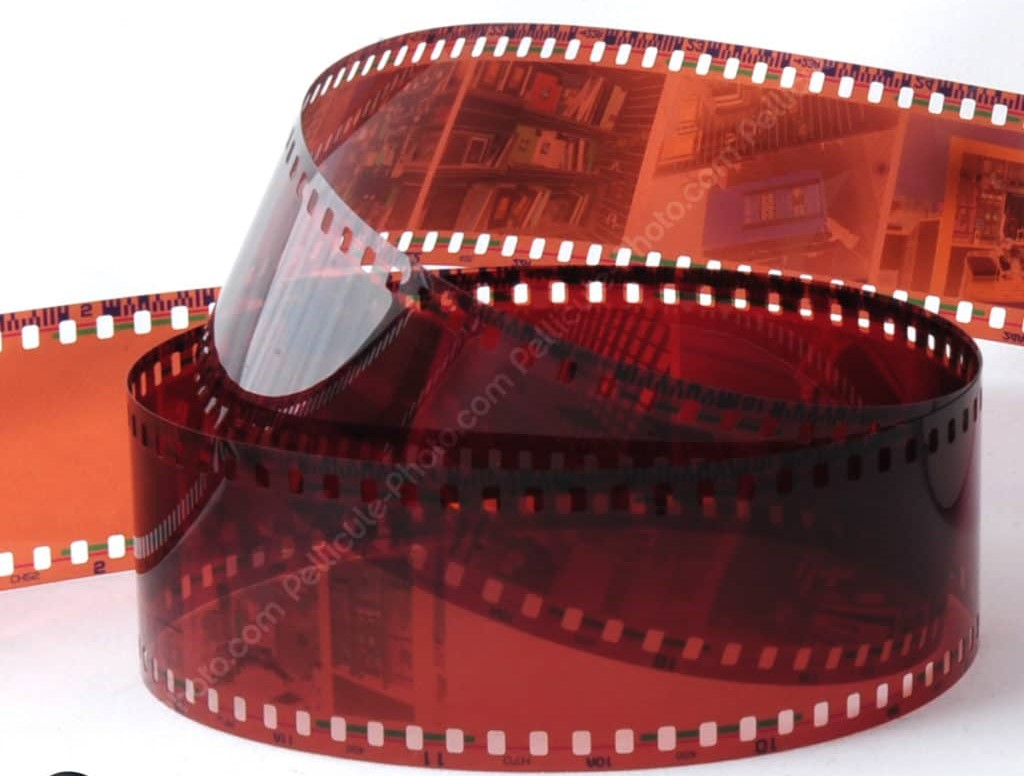
\includegraphics[scale=0.12]{images/pellicule.jpg}
 	}
 	\caption[Pellicule]{image d'une pellicule. source: https://lens.google.com}
 	\label{fig:Pellicule}
 \end{figure}
 
 
 Pour les types de caméra nous pouvons cité entre autre \cite{noauthor_les_2015} :
 
 \begin{itemize}
 	\item \textbf{Les caméras de smartphones} : Ce sont les caméras intégrés dans les téléphones portables.De nos jours la qualité des images qu'elles produisent les amènes à rivaliser avec les caméras professionnels qui existe sur le marché.Elles sont utilisés pour les web vidéos, clips, interviews, courts-métrages, etc......
 	
 	\item \textbf{Les Camescopes} sont des caméras utilisé par le grand public pour leurs souvenirs de famille.Aujord'hui elles sont rare sur le marché car elles sont remplacées par les smartphones.seuls les plus chers parviennent à se démarquer par leur qualité d’image . Elles sont souvent de petite taille, élaborées pour automatiser la plupart des réglages et disposent bien souvent de petits capteurs mais jamais d’entrées audio (Figure \ref{fig:Cmescopes}).
 	
 	\textbf{Exemple :}
 	
 	\begin{itemize}
 		\item Canon Vixia HF R52
 		\item Sony HDR PJ275
 		\item Panasonic HC W850
 	\end{itemize}
 	
 	\begin{figure}[H]%
 		\center%
 		\setlength{\fboxsep}{5pt}%
 		\setlength{\fboxrule}{0.5pt}%
 		\fbox{
 		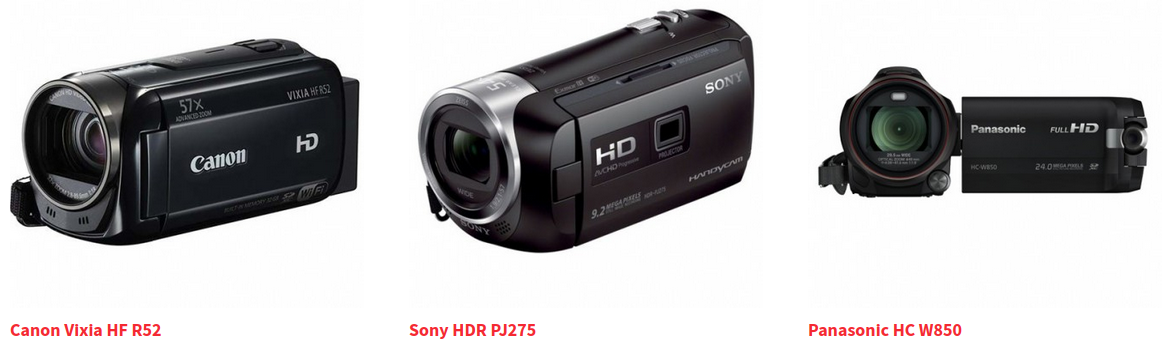
\includegraphics[scale=0.35]{images/camescopes.png}
 		}
 		\caption[Camescopes]{Les caméras de types camescopes. Source :\cite{noauthor_les_2015}}%
 		\label{fig:Cmescopes}
 	\end{figure}
 	
 	\item \textbf{Les DSLR(digital single-lens reflex)} sont des appareils photo réflex numériques disposant d’une fonction de capture vidéo.Ils sont caractérisés par la taille de leur capteur qui permettent d'avoir des images de qualités, d’objectifs interchangeables qui permettent de varier les rendus stylistiques en jouant avec les différents types de « cailloux » selon les photographes et la petite taille des lentilles (comparé à ceux d’une caméra pro) rend accessible le prix des objectifs (Figure \ref{fig:digital single-lens reflex(DSLR)}).
 	
 	\textbf{Exemple :}
 	
 	\begin{itemize}
 		\item Canon 5D Mark III
 		\item Nikon D800
 		\item Canon 7D
 	\end{itemize}
 	
 	\begin{figure}[H]%
 		\center%
 		\setlength{\fboxsep}{5pt}%
 		\setlength{\fboxrule}{0.5pt}%
 		\fbox{
 		 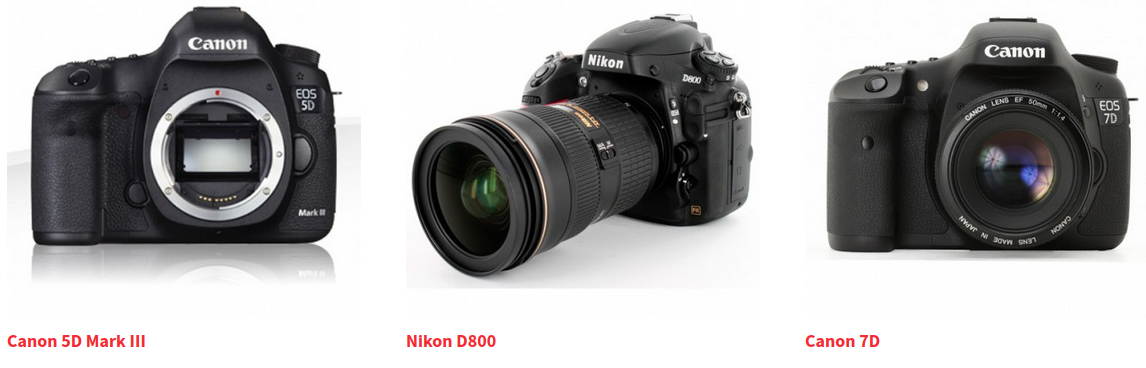
\includegraphics[scale=0.35]{images/DSLR.png}
 		}
 	 \caption[digital single-lens reflex(DSLR)]{Caméra digital single-lens reflex(DSLR). Source :\cite{noauthor_les_2015}}
 	\label{fig:digital single-lens reflex(DSLR)}
 	\end{figure}
 	
 	\item \textbf{Les Caméras dites « Prosommateurs »} Le mot « prosommateur » est composé de « pro » issu de production et « sommateur » de consommateur. On appelle les prosommateurs les personnes qui achètent des produits avec une certaine exigence car ils ont pour intention d’utiliser le produit dans un cadre de production.Ces caméras assez récentes sont venues perturber la frontière entre camescopes et caméras professionnelles en insérerant une gamme intermédiaire répondant aux besoins des petits producteurs indépendants.Elles sont généralement d’une taille supérieure à un camescope mais bien moins encombrante que les caméras pro de plateau ou de cinéma et proposent une excellente qualité d’image (Figure \ref{fig:Les Caméras dites « Prosommateurs »}).
 	
 	\textbf{Exemple :}
 	
 	\begin{itemize}
 		\item Sony PMW 300
 		\item Panasonic AG HPX250
 		\item Canon XF 205
 	\end{itemize}
  
  \begin{figure}[H]%
  	\center%
  	\setlength{\fboxsep}{5pt}%
  	\setlength{\fboxrule}{0.5pt}%
  	\fbox{
  			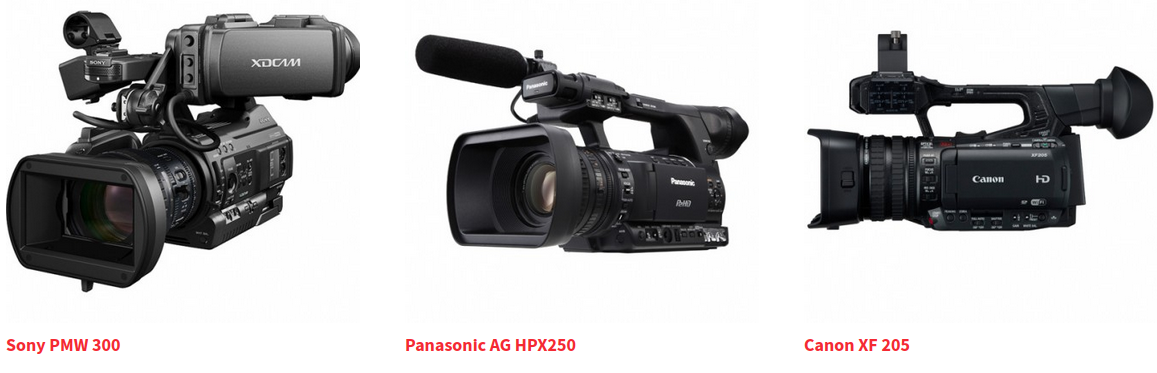
\includegraphics[scale=0.3]{images/prosommateur.png}
  	}
  \caption[Les Caméras dites « Prosommateurs »]{Les Caméras dites « Prosommateurs ». Source :\cite{noauthor_les_2015}}
  \label{fig:Les Caméras dites « Prosommateurs »}
  \end{figure}
  
 	\item \textbf{Caméras Professionnelles} Les caméras professionnelles sont de très grosses caméras disposant des capteurs les plus gros, les objectifs y sont évidemment interchangeables,le paramétrage de la colorimétrie y est bien souvent plus poussé, et elle sont systématiquement synchronisable par timecode (Figure \ref{fig:Caméras professionnel}).
 	
 	\textbf{Exemple :}
 	
 	\begin{itemize}
 		\item Panavision Panaflex Millenium
 		\item Arri Arriflex D-21
 		\item Aaton Penelope
 	\end{itemize}
 	
 	
 	\begin{figure}[H]%
 		\center%
 		\setlength{\fboxsep}{5pt}%
 		\setlength{\fboxrule}{0.5pt}%
 		\fbox{
 			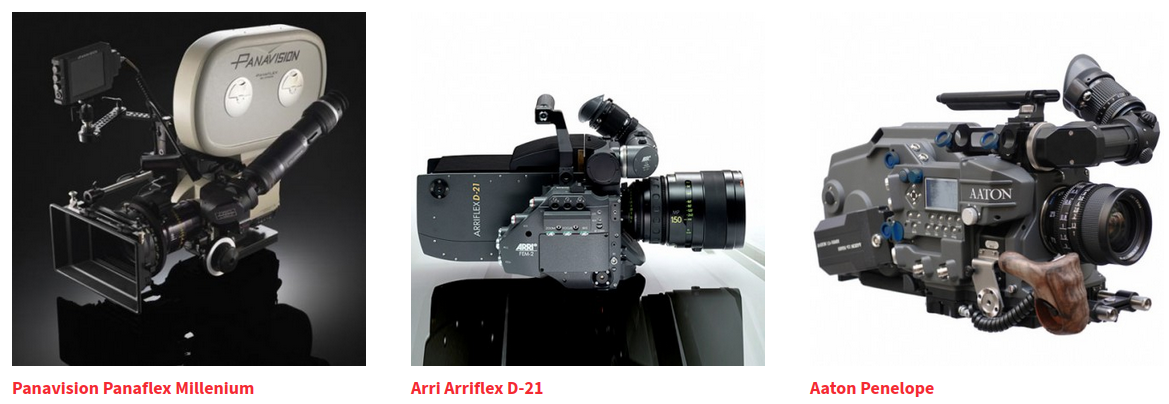
\includegraphics[scale=0.38]{images/professionnel.png}
 		}
 	\caption[Caméras professionnel]{Caméra  professionnel.Source :\cite{noauthor_les_2015}}
 	\label{fig:Caméras professionnel}
 	\end{figure}
 	
 	\item \textbf{Les Caméras de type "Super Concentré"} « Super Concentré » est un terme inventer dans l'article\cite{noauthor_les_2015} pour catégoriser cette dernière tendance d’appareils. Ce qui les qualifie c’est avant tout de très grands capteurs supérieurs à la majorité des caméras prosommateurs qui leur confère une qualité d’image cinématographique comparable aux caméras professionnelles. Les objectifs sont interchangeables, et sont capables d’exporter les rushs au format RAW qui permet une grande souplesse d’ajustement en post-prod (Figure \ref{fig:Caméras de type "Super Concentré"}).
 	
 	\textbf{Exemple :}
 	\begin{itemize}
 		\item Camera Red
 		\item Camera Blackmagic
 		\item Canon C300
 	\end{itemize}
 	 
 	 \begin{figure}[H]%
 	 	\center%
 	 	\setlength{\fboxsep}{5pt}%
 	 	\setlength{\fboxrule}{0.5pt}%
 	 	\fbox{
 	 		\includegraphics[scale=0.38]{images/super consentré.png}
 	 	}
 	 \caption[Caméras de type "Super Concentré" ]{Caméras de type "Super Concentré".Source :\cite{noauthor_les_2015}}
 	 \label{fig:Caméras de type "Super Concentré"}
 	 \end{figure}
 	 
 	\item \textbf{Les Caméras dédiées} sont des caméras qui sont particulièrement dédiées à un besoin spécifique comme les caméras miniatures pour les sports extremes ou l’embarcation dans les véhicules motorisés, les caméras à haute cadence pour le slow motion, les caméras 3D, ou encore les caméras drones (Figure \ref{fig:Caméras dedié}).
 	
 	\textbf{Exemple :}
 	
 	\begin{itemize}
 		\item Go Pro
 		\item Quadrirotor DJL Phantom 2 Vision
 		\item Hercules HD Twist
 		\item Panasonic AG 3DA1
 	\end{itemize}
 	
 	\begin{figure}[H]%
 		\center%
 		\setlength{\fboxsep}{5pt}%
 		\setlength{\fboxrule}{0.5pt}%
 		\fbox{
 		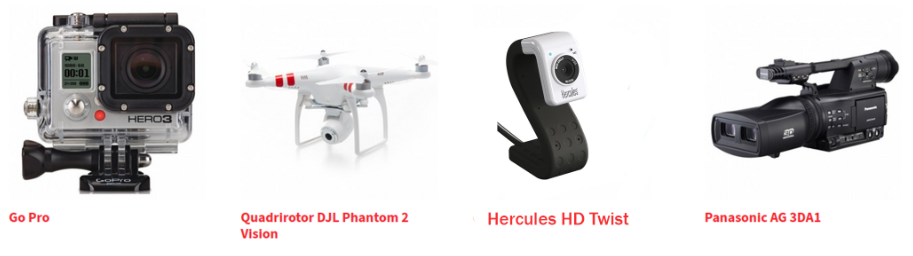
\includegraphics[scale=0.65]{images/caméras dedié.png}
 		}
 		\caption[Caméras dedié]{caméras dedié.Source :\cite{noauthor_les_2015}}
 	\label{fig:Caméras dedié}
 	\end{figure}
 	
 \end{itemize}
 
 Parmis ces différents types de caméra que nous avons cité , nous allons utilisé la caméra \textbf{Hercules HD Twist} qui est de type \textbf{dédiées}. Il possède un \textbf{Capteur CMOS HD 720p} qui capture des photo jusqu’à 5 Millions de pixels (interpolation logicielle) et de vidéo de 1280 x 720 pixels à 30 images par seconde. Il est équipé d'un microphone intégré avec réducteur de bruit,Un pied flexible en silicone et un câble USB 180 cm.
 %----------------------------------------------------------------------------------------
 %Notion de calibrage	
 %----------------------------------------------------------------------------------------
 \newpage
 
 
 \section{Notion de  Calibrage/étalonnage}\label{sec:Notion de  Calibrage/étalonnage}
 
 Le calibrage de caméra est un processus utilisé en vision par ordinateur et en traitement d'images pour estimer les paramètres intrinsèques et extrinsèques d'une caméra. Les paramètres intrinsèques comprennent des informations telles que la distance focale, le centre optique et les coefficients de distorsion, qui décrivent comment la caméra transforme les coordonnées 3D d'un point dans le monde réel en coordonnées 2D sur l'image capturée. Les paramètres extrinsèques décrivent la position et l'orientation de la caméra par rapport au monde réel.
 En calibrant une caméra, on peut compenser les distorsions optiques et géométriques qui peuvent affecter les images capturées. Cela est crucial pour des applications telles que la réalité augmentée, la cartographie 3D, la navigation robotique, la vision industrielle, la surveillance, etc.\\
 Ainsi calibrer une caméra consiste à estimer sa fonction de transfert \cite{orteu_calibrage_nodate} (Figure\ref{fig:Illustration caméras}).
 
 \begin{figure}[H]%
 	\center%
 	\setlength{\fboxsep}{5pt}%
 	\setlength{\fboxrule}{0.5pt}%
 	\fbox{
 		\includegraphics[scale=0.5]{images/illustration caméras.png}
 	}
   \caption[Illustration d'une caméras]{Schémas d'illustration d'une caméras. Source: \cite{orteu_calibrage_nodate}}
   \label{fig:Illustration caméras}
 \end{figure}
 
 Pour comprendre l'étalonnage de la caméra , il faut connaitre le modèle mathématique décrivant une caméra.
 Le modèle géométrique d’une caméra, représentée en Figure \ref{fig:Représentation du modèl sténopé}, est basé sur trois transformations élémentaires. Leur combinaison forme ce qu’on appelle le modèle sténopé ou « pinhole » en anglais \cite{eikosim_etalonnage_2021}.
 
  Ce modèle modélise une caméra par une projection perspective qui transforme un point 3D de l'espace en un point-image 2D,c'est une représentation mathématique d'un objet 3D projété dans un espace 2D\cite{orteu_calibrage_nodate}.\\
  Aussi connu sous le nom de "camera obscura" ou chambre noire,le modèle sténopé est un principe optique très ancien qui permet de capturer des images. Il est souvent utilisé pour expliquer les bases de la photographie et les principes fondamentaux de l'optique géométrique (Figure \ref{fig:Chambre Noir}) . 
 
  \begin{figure}[H]%
  	\center%
  	\setlength{\fboxsep}{5pt}%
  	\setlength{\fboxrule}{0.5pt}%
  	\fbox{
  	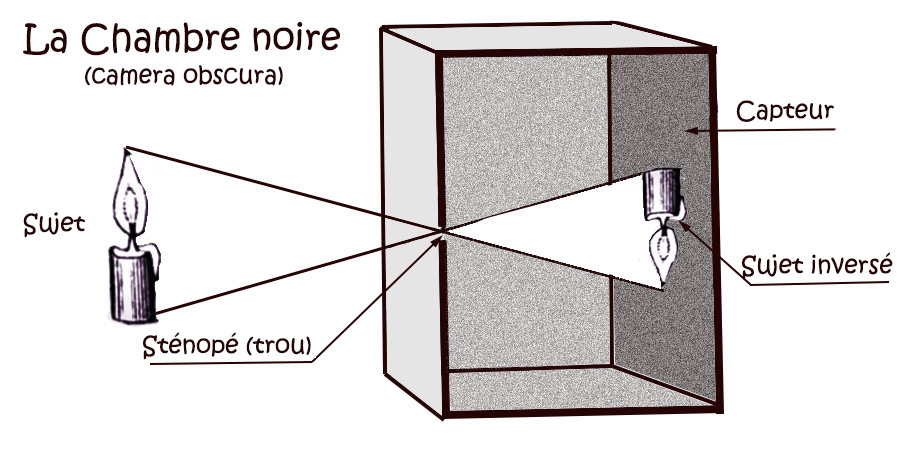
\includegraphics[scale=0.35]{images/chambre-noire.jpg}
  	}
  		\caption[Chambre Noir]{Chambre Noir ou Camera obscura. Source :https://lens.google.com}
  	\label{fig:Chambre Noir}
  \end{figure}
  
   \begin{figure}[H]%
  	\center%
  	\setlength{\fboxsep}{5pt}%
  	\setlength{\fboxrule}{0.5pt}%
  	\fbox{
  	 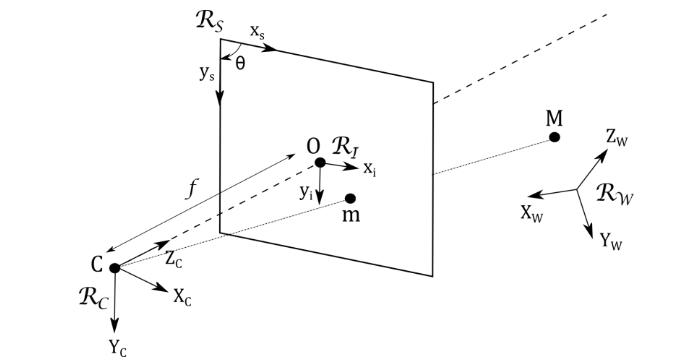
\includegraphics[scale=0.70]{images/modelstenope.png}
  	}
  	\caption[Représentation du modèl sténopé]{Projection d’un point 3D sur une image avec un modèle sténopé de caméra (adapté de \cite{eikosim_etalonnage_2021})}
    \label{fig:Représentation du modèl sténopé}
  \end{figure}
  
 
 La position d’un point 3D \textbf{M} de la scène, définie dans le repère monde $R_w$ par ses coordonnées ($X_w$, $Y_w$, $Z_w$), est exprimée dans le repère local $R_c$ attaché à la caméra \textbf{C} avec les coordonnées locales ($X_c$,$Y_c$,$Z_c$). Ce changement de repère constitue la première transformation et ne dépend que de trois rotations et de trois translations. Cette première transformation entre les coordonnées homogènes monde \{$X_w$\} = \{$X_w$, $Y_w$, $Z_w$,1\} et les coordonnées homogènes locales \{$X_c$\} = \{$X_c$, $Y_c$, $Z_c$,1\} est représentée par une matrice \textbf{4×4} notée \textbf{T}. Elle peut être décomposée en une matrice de rotation \textbf{R} (paramétrable par exemple par trois angles de rotation) et un vecteur de translation \textbf{t} (définie par trois composantes). On a donc:
 
 
 \begin{equation}
 \left\{
 \begin{array}{c}
 	X_c \\
 	Y_c\\
    Z_c \\
 	 1 \\
 \end{array}
 \right\}
 =
 \left[ \textbf{T} \right] 
 \left\{
 \begin{array}{c}
 	 X_w \\
 	 Y_w \\
 	 Z_w \\
 	 1 \\
 \end{array}
 \right\}
 =
 \left[  
 \begin{array}{cc}
\left[ \textbf{R} \right] & \{t\} \\
\{0_{1 \times 3}\} & 1 \\	 
 \end{array}
  \right] 
\left\{
\begin{array}{c}
	X_w \\
	Y_w \\
	Z_w \\
	1 \\
\end{array}
\right\}
=
 \left[ 
 \begin{array}{cccc}
 	r_{11} & r_{12} & r_{13} & t_x \\
 	r_{21} & r_{22} & r_{23} & t_y \\
 	r_{31} & r_{32} & r_{33} & t_z\\
 	0 & 0 & 0 & 1 \\
 \end{array}
  \right]
 \left\{
 \begin{array}{c}
 	X_w \\
 	Y_w \\
 	Z_w \\
 	1 \\
 \end{array}
 \right\}
  \end{equation}
 
  
 Ces six paramètres (trois angles, trois translations) sont appelés \textbf{paramètres extrinsèques} et définissent donc le positionnement de la caméra dans l’espace 3D.
 
 La deuxième transformation correspond à la projection du point 3D \textbf{M} sur le plan image auquel est attaché le repère local \textbf{$R_i$} en un point 2D \textbf{m}. Elle fait intervenir uniquement la focale \textbf{f} de la caméra et un facteur d’échelle \textbf{s} selon : 
 
 \begin{equation}
 s
 *
 \left\{
 \begin{array}{c}
 	x_i \\
 	y_i \\
 	z_i \\
 	1 \\
 \end{array}
 \right\}
 =
 \left[ 
  \begin{array}{cccc}
 	f & 0 & 0 & 0 \\
 	0 & f & 0 & 0 \\
 	0 & 0 & 1 & 0\\
 \end{array}
  \right]
  \left\{
  \begin{array}{c}
  	X_c \\
  	Y_c\\
  	Z_c \\
  	1 \\
  \end{array}
  \right\} 
\end{equation}
   
 La dernière transformation exprime les coordonnées 2D homogènes \{$x_s$\} = \{$x_s$, $y_s$, 1\}T du point projeté \textbf{m} dans le repère du capteur $R_s$ et fait intervenir les caractéristiques du capteur : 
 
 \begin{itemize}
 	\item l’angle de décadrage entre les axes horizontaux et verticaux du capteur (« skew »), supposé égal à 90° ;
 	\item la position du centre optique ;
 	\item la taille physique du pixel dans les deux directions.
 \end{itemize}
  
  La combinaison des deux précédentes transformations peut être décrite à travers une matrice de projection \textbf{3×4 K} qui s’écrit :
  
  \begin{equation}
  \left[ \textbf{K} \right] 
  =
  \left[ 
  \begin{array}{cccc}
  	f_x & 0 & c_x & 0 \\
  	0 & f_y & c_y & 0 \\
  	0 & 0 & 1 & 0\\
  \end{array}
  \right]
\end{equation}
  
  Cette matrice de projection est donc définie par quatre paramètres intrinsèques à la caméra étalonnée : les longueurs de focale horizontale $f_x$ et verticale $f_y$ en pixels et la position ($c_x$,$c_y$) en pixels du centre optique dans l’image.
  
  La matrice de projection complète \textbf{M} décrivant une caméra est donc composée d’une matrice de paramètres extrinsèques \textbf{T} et d’une matrice de paramètres intrinsèques \textbf{K}, de sorte que
  
   \begin{equation}
  s
  *
  \left\{ x_s \right\}
  =
  \left[ \textbf{K} \right] 
  \left[ \textbf{T} \right]
  \left\{ X_w \right\} 
  =
  \left[ \textbf{M} \right]
  \left\{ X_w \right\} 
\end{equation}
  
  La matrice de projection \textbf{M} peut ainsi être exprimée de façon « \textbf{implicite} » comme une matrice \textbf{3×4} contenant \textbf{12} termes ($m_{ij}$) ou bien de façon « \textbf{explicite} », via les \textbf{10} paramètres indépendants extrinsèques et intrinsèques présentés précédemment. Sous sa forme explicite, \textbf{M} s’écrit alors :
  
   \begin{equation}
  \left[ \textbf{M} \right]
  =
  \left[ 
  \begin{array}{cccc}
  	r_{11}f_x + r_{31}c_x & r_{12}f_x + r_{32}c_x & r_{13}f_x + r_{33}c_x & t_xf_x + t_zc_x \\
  	r_{21}f_y + r_{31}c_y & r_{22}f_y + r_{32}c_y & r_{23}f_y + r_{33}c_y & t_yf_y + t_zc_y \\
  	r_{31} & r_{32} & r_{33} & t_z\\
  \end{array}
  \right]
\end{equation}
  
  En globalité l'estimation des différents paramètres énumérés au dessus constitue le calibrage de la caméra.\\
  
  
  Plusieurs facteurs peuvent affecter la précision des résultats d’étalonnage de la caméra, mais la prise en compte de ces facteurs et l’utilisation de techniques d’étalonnage appropriées peuvent aider à garantir des résultats d’étalonnage précis et fiables de la caméra. \\
  
  Voici quelques-unes des plus importantes : 
  
  \begin{itemize}
  	\item \textbf{Distorsion de l’objectif } :  La distorsion de l’objectif peut entraîner des erreurs importantes dans le processus d’étalonnage de l’appareil photo. La distorsion se produit lorsque l’objectif projette le monde 3D sur le plan de l’image 2D, ce qui donne l’impression que les lignes droites sont incurvées. Les types courants de distorsion comprennent la distorsion radiale, qui provoque le gonflement de l’image vers l’extérieur ou vers l’intérieur, et la distorsion tangentielle, qui provoque l’inclinaison de l’image. Le calcul des coefficients de distorsion et leurs correction lors du calibrage aide à corriger ces erreurs  (Figure \ref{fig:Types de distorsion}). 
  	
  	\begin{figure}[h]
  		\centering
  		\fbox{
  			\begin{minipage}{0.24\textwidth}
  				\centering
  				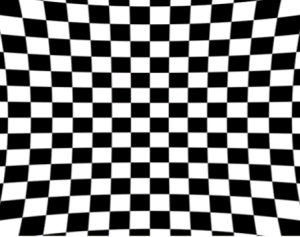
\includegraphics[width=\linewidth]{images/radialint}
  				\subcaption{(a)}
  			\end{minipage}\hfill
  			\begin{minipage}{0.25\textwidth}
  				\centering
  				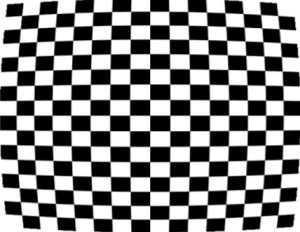
\includegraphics[width=\linewidth]{images/radialext}
  				\subcaption{(b)}
  			\end{minipage}\hfill
  			\begin{minipage}{0.26\textwidth}
  				\centering
  				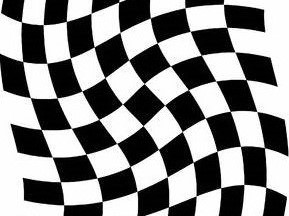
\includegraphics[width=\linewidth]{images/tang}
  				\subcaption{(c)}
  			\end{minipage}\hfill 
  		}
  		\caption[Types de distorsion]{(a)Distorsion radial intérieur, (b)Distorsion radial extérieur, (c) Distorsion tangentielle. Source :https://lens.google.com}
  		\label{fig:Types de distorsion}
  	\end{figure}
  	
  	\item \textbf{Résolution de l’image} : La résolution des images utilisées pour l’étalonnage de la caméra peut également affecter la précision des résultats. Les images haute résolution fournissent des informations plus détaillées sur le modèle d’étalonnage, ce qui peut conduire à des estimations plus précises de la matrice de projection de la caméra. Cependant, les images haute résolution nécessitent également plus de ressources de calcul et peuvent être plus difficiles à traiter.	\\
  	
  	\item \textbf{Placement de la caméra} : La position et l’orientation de la caméra peuvent également affecter la précision des résultats de l’étalonnage de la caméra. Les caméras doivent être placées à une distance suffisante du motif d’étalonnage pour s’assurer que la géométrie du motif est visible dans l’image. De plus, les caméras doivent être alignées parallèlement au motif pour minimiser la distorsion de perspective. \\
  	
  	\item \textbf{Qualité du modèle d’étalonnage} : la qualité du modèle d’étalonnage peut également affecter la précision des résultats d’étalonnage de la caméra. Les motifs d’étalonnage doivent être plats, rigides et avoir un contraste élevé pour garantir que la géométrie du motif est visible dans l’image. De plus, le motif doit être suffisamment grand pour couvrir tout le champ de vision de la caméra.\\
  	
  	\item \textbf{Nombre d'images} :  le nombre d’images utilisées pour l’étalonnage de la caméra peut également affecter la précision des résultats. L’utilisation d’un plus grand nombre d’images peut fournir plus d’informations sur la matrice de projection de la caméra, ce qui permet d’obtenir des estimations plus précises. Cependant, l’utilisation d’un trop grand nombre d’images peut également augmenter le coût de calcul du processus d’étalonnage. \\
  	
  	\item \textbf{Bruit et valeurs aberrantes} :  le bruit et les valeurs aberrantes dans les données d’image peuvent également affecter la précision des résultats d’étalonnage de la caméra. Le bruit peut introduire des erreurs aléatoires dans l’estimation de la matrice de projection de la caméra, tandis que les valeurs aberrantes peuvent introduire des erreurs systématiques. L’utilisation de techniques d’estimation robustes peuvent aider à atténuer les effets du bruit et des valeurs aberrantes.
  \end{itemize}
   
  
  
  
  
  
  
  
  
  
  
  \newpage
  
  %----------------------------------------------------------------------------------------
  %Approche de calibrage	
  %----------------------------------------------------------------------------------------
  \section{Approche de calibrage}
  
  De nombreux travaux ont été réalisés sur la notion de calibrage , à commencer par la communauté de la photogrammétrie et plus récemment en vision par ordinateur.
  Plusieurs approches existent qui peuvent être regroupées en trois grandes catégories, décrites ci-dessous : 
  
  \begin{itemize}[label={\Huge$\star$}]
  	 
  \item \textbf{L’étalonnage par mire}
  
  L’étalonnage par mire est donc basé sur l’utilisation d’un objet 3D de géométrie bien connue (appelé mire d’étalonnage) et son image acquise par la caméra. Cette mire présente sur sa surface des points 3D spécifiques, de positions connues . Ils peuvent correspondre à l’intersection de lignes verticales et horizontales quand la mire est une grille (ou un damier) ou bien au centre de cercles lorsque la mire est composée de points. La position de ces points 3D sur l’image de la mire est souvent obtenue via des procédures automatiques d’analyse d’images\cite{faugeras_three-dimensional_1993,eikosim_etalonnage_2021}  (Figure \ref{fig:Exemples de mires}).
  
  \begin{figure}[h]
  	\centering
  	\fbox{
  	\begin{minipage}{0.23\textwidth}
  		\centering
  		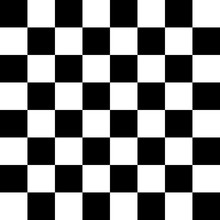
\includegraphics[width=\linewidth]{images/mire1}
  	\end{minipage}\hfill
  	\begin{minipage}{0.23\textwidth}
  		\centering
  		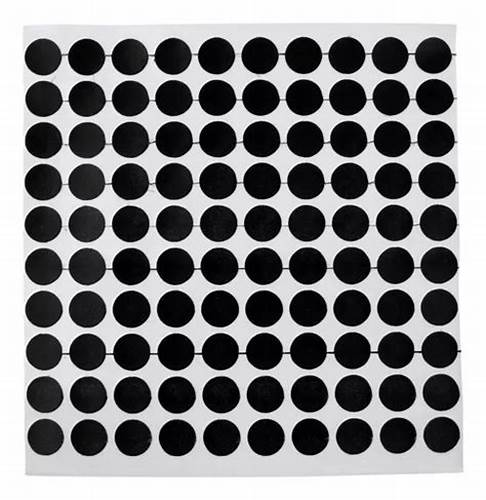
\includegraphics[width=\linewidth]{images/mire2}
  	\end{minipage}\hfill
  	\begin{minipage}{0.23\textwidth}
  		\centering
  		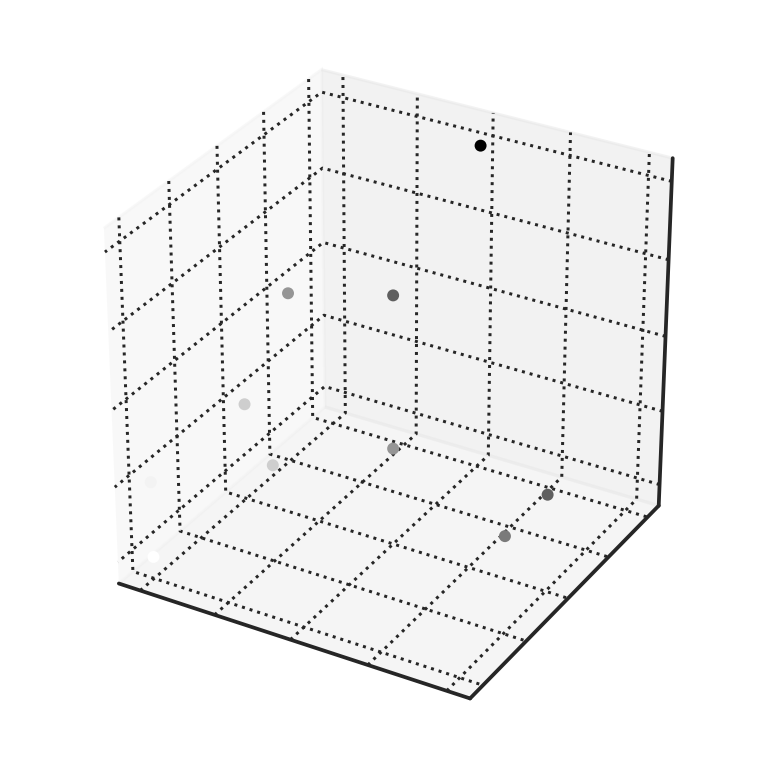
\includegraphics[width=\linewidth]{images/mire3}
  	\end{minipage}\hfill
  	\begin{minipage}{0.23\textwidth}
  		\centering
  		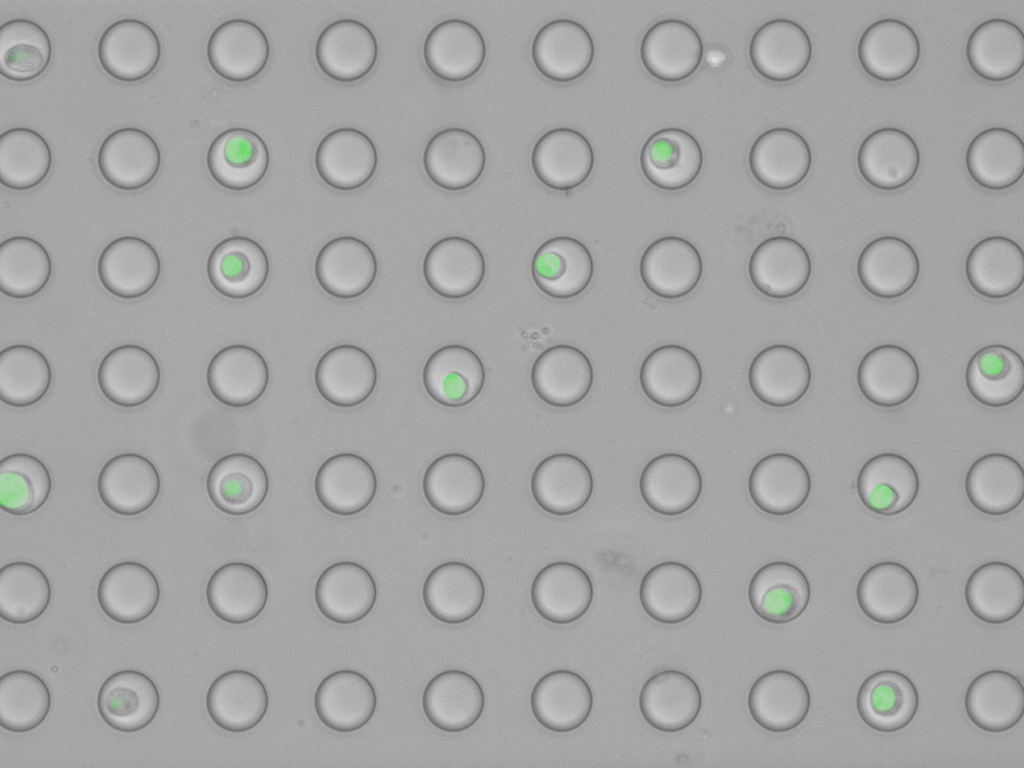
\includegraphics[width=\linewidth]{images/mire4}
  	\end{minipage}
  }
  \caption[Exemples de mires]{ Exemples de mires 3D et 2D présentant des motifs de grille et/ou de points. Source: https://lens.google.com}
  \label{fig:Exemples de mires}
  \end{figure}
  
  L’algorithme utilisé par cette approche vise alors à trouver les paramètres du modèle de caméra qui minimisent l’écart entre la position des points 3D projetés à l’aide du modèle de caméra et la position réelle de ces points sur l’image. L’algorithme consiste ainsi à optimiser la matrice de projection jusqu’à minimiser la somme quadratique de ces erreurs de reprojection. Avec ce type d’approche, la matrice de projection peut être identifiée soit de façon implicite, soit de façon explicite, et peut également inclure des modèles de distorsions pour les modèles les plus complexes. Dans le cas d’un système de stéréovision (c’est-à-dire à 2 caméras), cette approche va identifier de façon indépendante les paramètres (intrinsèques et extrinsèques) d’une des deux caméras, qui deviendra la « caméra maître ». La seconde caméra, dite « caméra esclave », aura ses paramètres intrinsèques identifiés via l’image de mire et ses paramètres extrinsèques seront définis par rapport à la position de la caméra maître, à travers la détermination d’une matrice de transformation linéaire permettant de passer de la caméra 1 à la caméra 2. Cette matrice peut être prédéfinie par le fournisseur de systèmes de stéréovision pour des systèmes où la position relative des caméras est fixée, ou réidentifiée à partir des images de mires. Les mires utilisées devant occuper un espace 3D, elles doivent être 3D ou bien, si elles sont planes, être déplacées dans l’espace selon des mouvements de translation et rotation. Avec ce type d’étalonnage, il est nécessaire de réaliser au moins une cinquantaine d’images de mire pour espérer pouvoir étalonner le système de stéréovision et minimiser l’effet du bruit d’acquisition et des erreurs d’étalonnage. De plus, la mire étant extérieure, il n’est pas possible de réétalonner les caméras au cours de l’essai, ce qui peut s’avérer nécessaire si les caméras bougent par inadvertance (déplacement des pieds de caméras, dévissage progressif des caméras…).
  Les méthodes couramment adoptées sont celles de Tsai \cite{tsai_versatile_1987}, Heikkila, Silven \cite{heikkila_four-step_1997} et Zhang \cite{zhengyou_zhang_flexible_1999}. Ceux-­ci sont tous basés sur le modèle de caméra sténopé et incluent des termes pour modéliser la distorsion radiale.
  
  \item \textbf{L’auto-étalonnage}
  
L’auto-étalonnage est utilisé en particulier par les approches de stéréocorrélation dites « globales », comme celle proposée par EikoTwin DIC \cite{noauthor_eikotwin_nodate}. Il utilise la pièce à tester dans son intégralité comme objet d’étalonnage et cela grâce à une description dense de l’objet (c’est-à-dire que la position de chaque point de la pièce est paramétrisée et peut être déterminée via un modèle mathématique). Parmi les descriptions possibles, on trouve celle du maillage par éléments finis. Ainsi, l’intégralité du maillage est utilisée comme points spécifiques pour minimiser les erreurs de reprojection et identifier les paramètres des modèles de caméra (et non plus uniquement les points particuliers d’une mire). A l’intégralité de ce maillage sera associée la totalité de la pièce mouchetée visible sur les images acquises par les caméras, et par extension toute la richesse de la texture de la pièce (mouchetis). La procédure a ainsi pour but de trouver simultanément les paramètres implicites paramétrisant les caméras (sans hiérarchisation entre les caméras), en minimisant l’écart en niveau de gris entre la projection des points 3D via chacune des caméras (à l’aide de son modèle de projection à optimiser) et une image de référence commune à toutes les caméras (construite à partir de toutes les caméras). Les points 3D correspondent à des points d’évaluation construits pour chaque élément du maillage (subdivisions équiréparties au sein de l’élément) où les niveaux de gris et gradients seront évalués pour minimiser les erreurs de reprojection. Ainsi, avec cette approche, il est possible d’étalonner un système de stéréovision avec une seule paire d’images tout en étant robuste au bruit grâce à la multiplicité des points d’évaluation induite par la description dense de la pièce d’essai. Par ailleurs, la position des caméras est exprimée dans le repère de la pièce et l’étalonnage étant basée sur cette dernière, il est possible de réétalonner à volonté les caméras au cours de l’essai en utilisant les images acquises\cite{eikosim_etalonnage_2021}.
  
  \item \textbf{L’étalonnage hybride}
  
  L’une des limitations de l'auto-étalonnage réside dans le caractère tridimensionnel de la pièce à tester, qui reste une condition pour éviter les singularités mathématiques de l’étalonnage d’une caméra. Pour les cas où la pièce ne respecte pas ces conditions géométriques (cas d’une pièce plane ou d’un solide de révolution tel que le cylindre), il est recommandé de procéder à un étalonnage dit « hybride », qui est également une procédure proposée par EikoTwin DIC \cite{noauthor_eikotwin_nodate,eikosim_etalonnage_2021}. Cette approche permet de combiner l’utilisation d’une mire de type ChAruCo (de géométrie bien connue) et une approche de stéréocorrélation globale (par auto-étalonnage). L’utilisation de la mire ChAruCo permet de fixer de façon explicite une partie des paramètres de projection, à savoir les paramètres intrinsèques de la caméra (matrice K), et de fiabiliser l’identification de la matrice extrinsèque T (sous forme implicite) par auto-étalonnage.
     
\end{itemize}

 
 En fonction des différents approches de calibrage et des facteurs qui peuvent affecter la précision des résultats que nous avons étudié précédemment , nous avons décider d'opter la méthode de \textbf{Zhang Zhengyou}\cite{zhengyou_zhang_flexible_1999} qui est le plus utiliser de nos jour et adaptable aux nouvelles domaines dont la vision par ordinateur.
 
 %----------------------------------------------------------------------------------------
 %Étude de la méthode de Zhang Zhengyou
 %----------------------------------------------------------------------------------------
 \section{Étude de la méthode de Zhang Zhengyou}
 
  
 La technique proposée proposé par zhang Zhengyou  \cite{zhengyou_zhang_flexible_1999} connue sous le nom de \textit{"méthode de calibrage de caméra basée sur le plan d'échiquier"} nécessite uniquement que la caméra observe un motif plan affiché dans quelques (au moins deux) orientations  différentes. Le motif peut être imprimé sur une imprimante laser et fixé  sur une surface plane « raisonnable » (par exemple, une couverture de livre rigide). La caméra ou le motif planaire peuvent être déplacés à la main.Par rapport aux techniques classiques, la technique proposée est considérablement plus flexible et par rapport à  l’auto-étalonnage, il gagne en robustesse.la nouvelle technique fait progresser la vision par ordinateur 3D des environnements de laboratoire au monde réel.
 
 Cette partie contient un résumé des parties essentiel de l'article selon notre compréhension. Pour plus de détaille voir
 \cite{zhengyou_zhang_flexible_1999}  
 
 La méthode se base sur la notation suivante qui respecte la géométrie du modèle sténopé abordé dans la section \ref{sec:Notion de  Calibrage/étalonnage}:
 
 Un point 2D est noté $m = [u, v]^{T}$ Un point 3D est noté $M = [X, Y, Z]^{T}$. On utilise $\bar{x}$ pour désigner le vecteur augmenté en ajoutant 1 comme dernier élément : $m =[u, v, 1]^{T}$ et $\bar{M} = [X, Y, Z, 1]^{T}$. Une caméra est modélisée par le sténopé habituel : la relation entre un point 3D M et sa projection d'image m est donnée par:
 
 
 \begin{equation}
 s\bar{m}= A\left[ 
 \begin{array}{cc}
 	R & t \\
 \end{array} \right]\bar{M}
 \hspace{1cm} 
  avec 
  \hspace{1cm} 
  A
  =
  \left[ 
  \begin{array}{ccc}
  	\alpha & c & u_0 \\
  	0 & \beta & v_0\\
  	0 & 0 & 1 \\
  \end{array} \right] 
  \label{eq:notation}
\end{equation}
   
   
 
 où \textbf{s} est un facteur d'échelle arbitraire ; \textbf{(R, t)} appelés paramètres extrinsèques, est la rotation et la translation qui relient le système de coordonnées mondiales au système de coordonnées de la caméra ; \textbf{A} est appelée la matrice intrinsèque de la caméra, et $(u_0, v_0)$ sont les coordonnées du point principal, $\alpha$ et $\beta $  l'échelle facteurs dans l'image des axes u et v et c le paramètre décrivant l'asymétrie des deux axes de l'image.\\
 Nous utilisons l'abréviation $m = A^{-T}$ pour
 $(A^{-1})^{T}$ ou $(A^{T})^{-1}$
 
  Un point modèle \textbf{M} et son image \textbf{m} sont liés par une homographie \textbf{H} :
  
\begin{equation} 
 s\bar{m}=H\bar{M}
 \hspace{1cm} 
 avec
 \hspace{1cm} 
 H=A
 \left[ 
 \begin{array}{ccc}
 	r_1 & r_2 & t\\
 \end{array} \right]
 \label{eq:homographie}
\end{equation}
 
 
 
 En fonction cette notation et  l'homographie lié au modèle sténopé nous avons pu voir les contraintes de base liées aux paramètres intrinsèques lors de l'observation d'un seul plan qui sont entre autre:  
 
 \begin{equation} 
 h_{1}^{T} 
 A^{-T}
 A^{-1}
 h_2
 \label{eq:contrainte1}
 \end{equation}
 
 \begin{equation} 
 h_{1}^{T} 
 A^{-T}
 A^{-1}
 h_1
 =
 h_{2}^{T} 
 A^{-T}
 A^{-1}
 h_2
 \label{eq:contrainte2}
 \end{equation}
 
 Pour résoudre de manière efficace le problème d'étalonnage de la caméra, l'article a abordé d'abord la solution fermé qui permet de résoudre les contraintes liées aux paramètres intrinsèques , ensuite la technique d'optimisation non linéaire basée sur le critère du maximum de vraisemblance pour affiner les paramètres avec l'algorithme de Levenberg ­Marquardt et enfin la prise en compte de la distorsion radial de la lentille pour corriger la distorsion. \\
 
 \begin{itemize}[label={\Huge$\star$}]
 	\item \textbf{La solution fermé}
 	\\
 	
 	prenons 
 	
 	\begin{equation}
 	B
 	=
 	A^{-T}
 	A^{-1}
 	\equiv
 	\left[ 
 	\begin{array}{ccc}
 		B_{11} & B_{12} & B_{13} \\
 		B_{12} & B_{22} & B_{23}\\
 	    B_{13} & B_{23} & B_{33} \\
 	\end{array} \right]
 	\label{eq:solution fermé1}
 	\end{equation}
 	
 Notez que B est symétrique, défini par un vecteur 6D
 
\begin{equation}
 b
 =
 \left[ 
 \begin{array}{cccccc}
B_{11} & B_{12}  & B_{22} & B_{13} & B_{23} & B_{33}\\
 \end{array} \right]^{T}
\label{eq:solution fermé 2}
\end{equation}
 	
 Nous avons ensuite
 \begin{equation}
  h_{i}^{T}Bh_{i}
  =
  v_{ij}^{T}b
  \label{eq:solution fermé 3}
\end{equation}
  
  Ainsi, les deux contraintes fondamentales \ref{eq:contrainte1} et \ref{eq:contrainte2}, à partir d'une 
  homographie donnée, peuvent être réécrites sous la forme de 2 équations homogènes en b :	
  
 \begin{equation}
  \left[ 
  \begin{array}{c}
  	 v_{12}^{T} \\
  	 (v_{11}-v_{22})^{T}\\
  \end{array} \right]b
  =
  0
\label{eq:solution fermé 4}
\end{equation}

 Si n images du plan modèle sont observées, en empilant n équations nous avons :
 
  \begin{equation}
 v_b = 0
 \label{eq:solution fermé 5}
 \end{equation}
 
 où V est une matrice 2n × 6. 
 
Si $n \geq 3$, on aura en général une unique solution b définie à un facteur d'échelle près.
Si n = 2, nous pouvons imposer la contrainte asymétrique c = 0 , ce qui signifie que $[0, 1, 0, 0, 0, 0]b = 0$, qui est ajoutée comme équation supplémentaire à \ref{eq:solution fermé 5}. La solution de \ref{eq:solution fermé 5} est bien connue sous le nom de vecteur propre de $V^{T}V$ associé à la plus petite valeur propre (de manière équivalente, le vecteur singulier droit de V associé à la plus petite valeur singulière)
 
 Une fois b estimé, nous pouvons calculer la matrice intrinsèque \textbf{A} de la caméra.  
 Les paramètres extrinsèques de chaque image sont facilement calculé grâce à la matrice  intrinsèque \textbf{A}.
 
 De \ref{eq:homographie},on a: 
 \[
 r_{1}=\lambda A^{-1}h_{1}
 r_{2}=\lambda A^{-1}h_{2}
 r_{3}=r_{1}*r_{2}
 t=\lambda A^{-1}h_{3}
 \]
 
 
\item \textbf{Estimation de vraisemblance maximale} 
 \\
 
 La solution ci-dessus est obtenue en minimisant une distance 
 algébrique qui n'a pas de signification physique. Nous pouvons l’affiner 
 grâce à l’inférence du maximum de vraisemblance.
 On nous donne n images d’un plan modèle et il ya m points sur le 
 plan modèle. Supposons que les points images soient corrompus par un 
 bruit indépendant et identiquement distribué.
 L'estimation du maximum de vraisemblance peut être obtenue en minimisant la fonctionnelle suivante :
 
 \begin{equation}
 \sum_{i=1}^{n} \sum_{j=1}^{m} 
 ||m_{ij}-\hat{m}(A,R_{i},t_{j},M_{j})||^{2}
 \label{eq:maximum}
\end{equation}
 
 où $\hat{m}(A,R_{i},t_{j},M_{j})$est la projection du point $M_{j}$  dans l'image i, selon l'équation \ref{eq:homographie}. Une rotation R est paramétrée par un vecteur de 3 paramètres noté r qui est parallèle à l'axe de rotation et dont l'amplitude est égale à l'angle de rotation.  
 
 La minimisation  \ref{eq:maximum} est un problème de minimisation non 
 linéaire, qui est résolu avec l'algorithme de Levenberg-Marquardt tel 
 qu'implémenté dans Minpack \cite{watson_levenberg-marquardt_1978}. Cela nécessite une estimation initiale 
 de \textbf{A}, $\{R_i, t_i|i = 1..n\}$ qui peut être obtenue en utilisant la technique 
 décrite dans la sous-section précédente.\\
 
 \item \textbf{Prise en compte de la distorsion radial}
 \\
 
 Jusqu’à présent, nous n’avons pas pris en compte la distorsion de l’objectif 
  de la caméra. Cependant, une caméra de bureau présente généralement 
 une distorsion d'objectif importante, en particulier une distorsion radiale. 
  D'après quelques littérature, il est probable que la fonction de distorsion soit totalement dominée par les 
 composantes radiales, et surtout dominée par le premier terme Il a également été constaté qu'une modélisation plus élaborée non seulement n'aiderait pas (négligeable par rapport à la quantification du 
 capteur), mais entraînerait également une instabilité numérique.
 
 on a les équations résultante suivant:
 
 \begin{equation}
 	k
 	=
 	(D^{T}D)^{-1}D^{T}d
 	\label{eq:radial}
 \end{equation}	
 	
 	\begin{equation}
 		\sum_{i=1}^{n} \sum_{j=1}^{m} 
 		||m_{ij}-\mathring{m}
 		(A,R_{i},t_{j},M_{j})||^{2}
 		\label{eq:radial2}
 	\end{equation}
 	
 \end{itemize} 
 
 Les algorithmes proposées par Burger Wilhelm nous a permit d'avoir plus de détaille et de compréhension sur la méthode de Zhang \cite{burger_zhangs_2016}.
 
%----------------------------------------------------------------------------------------
%Notion de mesure de distance numériques
%----------------------------------------------------------------------------------------


\newpage
\section{Mesure de distance à l'aide d'une caméra}

La mesure de distance à l'aide d'une caméra est devenue une composante essentielle de nombreuses technologies modernes, offrant des solutions précises et polyvalentes pour évaluer la séparation spatiale entre les objets et l'observateur. Cette méthode, reposant sur les principes de la géométrie, de la physique optique et de l'analyse d'image, joue un rôle crucial dans une multitude de domaines.  
L'évolution rapide des capteurs d'imagerie et des algorithmes de traitement d'image a permis des avancées significatives dans la précision et la fiabilité de la mesure de distance avec les caméras. Cette technologie repose sur des fondements solides, exploitant des concepts tels que la parallaxe, la triangulation et la propagation de la lumière pour estimer les distances avec une précision remarquable.
La mesure de distance à l'aide d'une caméra offre une variété de techniques, allant de la stéréovision à la triangulation laser en passant par la mesure de temps de vol. Chacune de ces méthodes présente ses propres avantages et limitations, mais toutes partagent l'objectif commun d'obtenir des mesures précises dans des environnements divers et changeants.

 \begin{itemize}[label={\Huge$\star$}]
 	
 	\item \textbf{Stéréovision :}
 	
 	La stéréovision repose sur le principe de la vision binoculaire, similaire à la manière dont fonctionnent les yeux humains pour percevoir la profondeur. Cette technique utilise deux caméras placées à des positions légèrement différentes pour capturer des images de la même scène. En comparant les différences entre ces deux images, telles que les disparités de pixels, il est possible de déterminer la profondeur et la distance des objets dans la scène. Plus précisément, la stéréovision utilise la triangulation pour calculer la distance, en mesurant les angles et les proportions entre les points d'intérêt dans les images capturées par les deux caméras. Cette méthode offre une mesure de distance précise et robuste, mais elle nécessite un calibrage précis des caméras et peut être sensible aux variations d'éclairage et aux occlusions. Cette technique a été plus abordé dans \cite{adil_novel_2022} où l’article présente un algorithme basé sur Python pour mesurer la distance.Les expériences montrent que l’algorithme peut mesurer la distance avec une précision allant jusqu’à 99.83\% et un temps de traitement inférieur à 0.355 secondes pour des obstacles positionnés à des distances de 60 à 200 cm.
 	
 	\item \textbf{Triangulation laser}
 	
 	La triangulation laser utilise un faisceau laser pour projeter une lumière sur l'objet dont la distance doit être mesurée. Cette lumière réfléchie est ensuite capturée par une caméra, et la position du point lumineux sur l'image est analysée pour calculer la distance. La triangulation repose sur le principe de la géométrie triangulaire, où la distance est calculée en mesurant l'angle entre le faisceau laser, la caméra et le point réfléchi sur l'objet. Cette technique est souvent utilisée dans les applications nécessitant une grande précision, comme la métrologie industrielle et la cartographie 3D. Cependant, elle peut être sensible aux conditions d'éclairage et nécessite un alignement précis entre le faisceau laser et la caméra pour des mesures précises.
 	
 	\item \textbf{Mesure de temps de vol }
 	
 	La mesure de temps de vol est une méthode directe pour mesurer la distance entre la caméra et l'objet en utilisant la vitesse de la lumière. Cette technique implique l'envoi d'impulsions lumineuses de courte durée vers l'objet, puis la mesure du temps qu'il faut pour que ces impulsions rebondissent sur l'objet et reviennent à la caméra. En utilisant la vitesse de la lumière connue, il est possible de calculer la distance parcourue par les impulsions lumineuses et donc la distance entre la caméra et l'objet. La mesure de temps de vol est rapide, précise et fonctionne bien dans diverses conditions d'éclairage. Elle est souvent utilisée dans les applications telles que la détection d'obstacles pour les véhicules autonomes, la réalité augmentée et les systèmes de surveillance. Cependant, cette méthode peut être limitée par sa portée maximale et sa sensibilité aux surfaces réfléchissantes.

 \end{itemize}

Ce pendant dans ces différents techniques, la précision de la mesure dépend de plusieurs facteurs, notamment la qualité de l'image, le calibrage de la caméra, les conditions d'éclairage et la présence d'obstacles. Une résolution d'image plus élevée et un bon calibrage de la caméra sont essentiels pour une mesure précise. Les conditions d'éclairage peuvent affecter la qualité de l'image, tandis que la présence d'obstacles peut perturber les mesures, en particulier dans les environnements encombrés.\\

Parmis ces tehniques la stéréovision est la plus adapté pour notre projet mais comme nous avons une seule caméra à notre disposition ,nous avons utilisé une methode de mesure de distance basée sur des méthodes de détection d'objets ou de détection de contours et de calcul de distance à partir de la taille des objets dans une image prise après le saut.


\newpage
\section{CONCLUSION}

En conclusion, ce chapitre a exploré en profondeur les concepts clés liés au calibrage de caméra et à son application à l'estimation de performances lors de sauts en longueur. Nous avons commencé par définir les termes clés tels que la caméra, le calibrage et la mesure de distance à l'aide d'une caméra, soulignant leur importance dans le processus d'acquisition d'images et de mesure de distances précises.

Le calibrage de caméra, en particulier, a été identifié comme une étape cruciale pour corriger les distorsions, ainsi que pour établir une relation précise entre les coordonnées des pixels dans l'image et les coordonnées du monde réel.  

En intégrant des techniques de mesure de distance à l'aide d'une caméra, telles que la stéréovision ou la triangulation, avec un calibrage précis de la caméra, il est possible d'obtenir des estimations fiables de la distance parcourue lors d'un saut en longueur. Cette approche offre une alternative précise et non invasive aux méthodes traditionnelles de mesure de performances, permettant une évaluation objective et détaillée des performances athlétiques.
 